%
% file : descrption.tex
% date : samedi 11 janvier 2020, 12:24:22 (UTC+0100)
% author : sedelpeuch
% description :
\documentclass[a4paper,10pt]{report}
\usepackage[utf8]{inputenc}
\usepackage[T1]{fontenc}
\usepackage[french]{babel}
\usepackage{graphicx}
\usepackage{ulem}
\usepackage{float}
\usepackage{amsmath}
\usepackage{amssymb}
\usepackage{mathrsfs}
\usepackage{color}
\usepackage{fancyhdr}
\usepackage{pdfpages}
\usepackage{layout}
\usepackage{multicol}
\usepackage{setspace}
\usepackage{tabularx,array}
\usepackage[colorlinks=true]{hyperref}
\usepackage{tikz, tkz-tab}
\usepackage[top=2cm,bottom=2cm,left=2cm,right=2cm]{geometry}
\usepackage{amsthm}
\usepackage{listings}
\setlength{\parindent}{1cm}
\setlength{\parskip}{1ex plus 0.5ex minus 0.2ex}
\newcommand{\hsp}{\hspace{20pt}}
\newcommand{\HRule}{\rule{\linewidth}{0.5mm}}


\begin{document}
\begin{spacing}{1.5}
\graphicspath{{../reunion/}}
\begin{titlepage}
\begin{sffamily}
\begin{center}
\vspace*{\stretch{1}}
\textsc{\LARGE Eirbot \\ Coupe de France de robotique}\\[2cm]
\HRule \\[0.4cm]
{\huge \bfseries Equipe Eirboat \\[0.4cm]}

\HRule \\[2cm]

\textsc{\Large 1A 2019-2020}\\[2cm]
              
\includegraphics[scale=0.3]{LogoEirbot.png} \vfill

\vspace*{\stretch{1}}
  \end{center}
  \end{sffamily}
\end{titlepage}
\setcounter{tocdepth}{2}
\tableofcontents
\newpage
\pagestyle{fancy}
\lhead{Eirbot 1A}
\chead{\textbf{Description du projet}}
\rhead{\thepage}
\lfoot{2019-2020}
\cfoot{Equipe Eirboat}
 \fancyfoot[R]
 {
 
\includegraphics[scale=0.075]{65508.png}
 }

 \setcounter{part}{1}
\part{Description des projets}
\chapter{Description générale de l'organisation}
Ce chapitre a pour but de mettre en place l'organisation générale du travail. Il
faut comprendre que lors de cette division nous nous connaissions peu. Ce genre
de brain storming nous a alors appris à nous connaitre et à définir gloablement
les objectifs du robot.
\section{Arbres des tâches à réaliser par le robot}
Dans un premier temps nous réalisons un schéma des différentes tâches à
effectuer par le robot. Ces dernières nous permettrons de cadrer le robot et
plutard de mettre en place la stratégie de ce dernier.
\label{taches}
\HRule
\begin{center}
\begin{tikzpicture}
\tikzstyle{lien}=[->,>=stealth,rounded corners=20pt,thick]
\tikzset{individu/.style={draw,thick,fill=#1!25},
individu/.default={white}}
\node[individu=blue] (A) at (0,0) {\textsc{Se mouvoir}};
\node[individu] (A1) at (-7,-2) {Odométrie};
\node[individu] (A2) at (-3,-2) {Moteurs Maxon};
\node[individu] (A3) at (7,-2) {Asservissement};
\node[individu] (A3b) at (7,-4) {Encodeur};
\node[individu] (A4) at (3,-2) {\xout{Roue folle 2 roues motrices}};
\node[individu] (A5) at (3,-4) {2 roues motrice + patins};

\draw[lien] (A) -- (A1);
\draw[lien] (A) -- (A2);
\draw[lien] (A) -- (A3);
\draw[lien] (A) -- (A4);
\draw[lien] (A3) -- (A3b);
\draw[lien] (A4) -- (A5);


\end{tikzpicture}
\end{center}

\begin{center}
\begin{tikzpicture}
\tikzstyle{lien}=[->,>=stealth,rounded corners=20pt,thick]
\tikzset{individu/.style={draw,thick,fill=#1!25},
individu/.default={white}}
\node[individu=blue] (A) at (0,0) {\textsc{Mécanique générale}};
\node[individu] (A1) at (-3,-2) {Structure octogonale};
\node[individu] (A2) at (0,-2) {Profilés};
\node[individu] (A3) at (3,-2) {Etage rectangulaire};

\draw[lien] (A) -- (A1);
\draw[lien] (A) -- (A3);
\draw[lien] (A) -- (A2);

\end{tikzpicture}
\end{center}
\HRule
\begin{multicols}{2}
\begin{center}
\begin{tikzpicture}
\tikzstyle{lien}=[->,>=stealth,rounded corners=20pt,thick]
\tikzset{individu/.style={draw,thick,fill=#1!25},
individu/.default={white}}
\node[individu=red] (A) at (0,0) {\textsc{Détecter adversaire}};
\node[individu] (A1) at (0,-2) {Capteurs};
\node[individu] (A1a) at (-2,-4) {\xout{Ultrasons}};
\node[individu] (A1b) at (2,-4) {Infra rouge};

\draw[lien] (A) -- (A1);
\draw[lien] (A1) -- (A1a);
\draw[lien] (A1) -- (A1b);

\end{tikzpicture}
\end{center}
\columnbreak
\begin{center}
\begin{tikzpicture}
\tikzstyle{lien}=[->,>=stealth,rounded corners=20pt,thick]
\tikzset{individu/.style={draw,thick,fill=#1!25},
individu/.default={white}}
\node[individu=red] (A) at (0,0) {\textsc{Détecter Objet}};
\node[individu] (A1) at (-2,-2) {Couleur écocup};
\node[individu] (A1a) at (-2,-4) {Capteurs RGB};\node[individu] (A2) at (2,-2) {Pendant le ramassage};

\draw[lien] (A) -- (A1);
\draw[lien] (A1) -- (A1a);
\draw[lien] (A) -- (A2);
\draw (-3,0) -- (3,-4);
\draw (3,0) -- (-3,-4);


\end{tikzpicture}
\end{center}
\end{multicols}

\begin{multicols}{2}
\begin{center}
\begin{tikzpicture}
\tikzstyle{lien}=[->,>=stealth,rounded corners=20pt,thick]
\tikzset{individu/.style={draw,thick,fill=#1!25},
individu/.default={white}}
\node[individu=red] (A) at (0,0) {\textsc{Lire boussole}};
\node[individu] (A1) at (-2,-2) {Capteur};
\node[individu] (A1a) at (-2,-4) {Webcam};\node[individu] (A2) at (2,-2) {Balise sur le côté};

\draw[lien] (A) -- (A1);
\draw[lien] (A1) -- (A1a);
\draw[lien] (A) -- (A2);

\end{tikzpicture}
\end{center}
\columnbreak
\begin{center}
\begin{tikzpicture}
\tikzstyle{lien}=[->,>=stealth,rounded corners=20pt,thick]
\tikzset{individu/.style={draw,thick,fill=#1!25},
individu/.default={white}}
\node[individu=red] (A) at (0,0) {\textsc{Communication}};
\node[individu] (A1) at (-2,-2) {InfraRouge};;\node[individu] (A2) at (2,-2) {Bluetooth};

\draw[lien] (A) -- (A1);
\draw[lien] (A) -- (A2);

\end{tikzpicture}
\end{center}
\end{multicols}
\HRule

\begin{multicols}{2}
\begin{center}
\begin{tikzpicture}
\tikzstyle{lien}=[->,>=stealth,rounded corners=20pt,thick]
\tikzset{individu/.style={draw,thick,fill=#1!25},
individu/.default={white}}
\node[individu=green] (A) at (0,0) {\textsc{Elévation drapeau}};
\node[individu] (A1) at (-2,-2) {Timer};
\node[individu] (A2) at (2,-2) {Servomoteurs};

\draw[lien] (A) -- (A1);
\draw[lien] (A) -- (A2);

\end{tikzpicture}
\end{center}
\columnbreak
\begin{center}
\begin{tikzpicture}
\tikzstyle{lien}=[->,>=stealth,rounded corners=20pt,thick]
\tikzset{individu/.style={draw,thick,fill=#1!25},
individu/.default={white}}
\node[individu=green] (A) at (0,0) {\textsc{Manche à air}};
\node[individu] (A1) at (-2,-2) {Servomoteurs};
\node[individu] (A2) at (2,-2) {Coupler activation phare};

\draw[lien] (A) -- (A1);
\draw[lien] (A) -- (A2);

\end{tikzpicture}
\end{center}
\end{multicols}
\HRule

\begin{center}
\begin{tikzpicture}
\tikzstyle{lien}=[->,>=stealth,rounded corners=20pt,thick]
\tikzset{individu/.style={draw,thick,fill=#1!25},
individu/.default={white}}
\node[individu=gray] (A) at (0,0) {\textsc{Cartes}};
\node[individu] (A1) at (-4,-2) {Carte de puissance};
\node[individu] (A2) at (0,-2) {Carte de sécurité};
\node[individu] (A3) at (4,-2) {Carte d'alimentation};

\draw[lien] (A) -- (A1);
\draw[lien] (A) -- (A2);
\draw[lien] (A) -- (A3);


\end{tikzpicture}
\end{center}
\HRule

\begin{center}
\begin{tikzpicture}
\tikzstyle{lien}=[->,>=stealth,rounded corners=20pt,thick]
\tikzset{individu/.style={draw,thick,fill=#1!25},
individu/.default={white}}
\node[individu=orange] (A) at (0,0) {\textsc{Phare}};
\node[individu] (A1) at (-6,-2) {Elévation};
\node[individu] (A1a) at (-8,-4) {Bras robot};
\node[individu] (A1b) at (-4,-4) {\xout{Crémaillère}};
\node[individu] (A2) at (0,-2) {Activation};
\node[individu] (A2a) at (-1,-4) {\xout{Ddp}};
\node[individu] (A2b) at (1,-4) {Boutons};
\node[individu] (A3) at (6,-2) {Lumière};
\node[individu] (A3a) at (5,-4) {Ruban LED};
\node[individu] (A3b) at (7,-4) {\xout{Projo}};

\draw[lien] (A) -- (A1);
\draw[lien] (A1) -- (A1a);
\draw[lien] (A1) -- (A1b);
\draw[lien] (A) -- (A2);
\draw[lien] (A2) -- (A2a);
\draw[lien] (A2) -- (A2b);
\draw[lien] (A) -- (A3);
\draw[lien] (A3) -- (A3a);
\draw[lien] (A3) -- (A3b);


\end{tikzpicture}
\end{center}
\HRule

\newpage
\section{Répartition des tâches}
Dans un second temps nous nous répartissons de manière globale les tâches à
réaliser. \\
\label{repartition}
\HRule
\begin{center}
\begin{tikzpicture}
\tikzstyle{lien}=[->,>=stealth,rounded corners=20pt,thick]
\tikzset{individu/.style={draw,thick,fill=#1!25},
individu/.default={white}}
\node[individu=blue] (A) at (0,0) {\textsc{Se mouvoir} Carte puissance};
\node[individu] (A1) at (-3,-2) {Martin};
\node[individu] (A2) at (-1,-2) {\xout{Julien}};
\node[individu] (A3) at (1,-2) {\xout{Valentin}};
\node[individu] (A4) at (3,-2) {Filipe};

\draw[lien] (A) -- (A1);
\draw[lien] (A) -- (A2);
\draw[lien] (A) -- (A3);
\draw[lien] (A) -- (A4);


\end{tikzpicture}
\end{center}
\begin{center}
\begin{tikzpicture}
\tikzstyle{lien}=[->,>=stealth,rounded corners=20pt,thick]
\tikzset{individu/.style={draw,thick,fill=#1!25},
individu/.default={white}}
\node[individu=blue] (A) at (0,0) {\textsc{Se mouvoir} Odométrie, Asservissement
\& Haut niveau};
\node[individu] (A1) at (-5,-2) {\xout{Raphaël}};
\node[individu] (A2) at (0,-2) {Clément};
\node[individu] (A3) at (5,-2) {SD};
\node[individu] (A4) at (-3,-2) {Emile};
\node[individu] (A5) at (3,-2) {Liam};

\draw[lien] (A) -- (A1);
\draw[lien] (A) -- (A2);
\draw[lien] (A) -- (A3);
\draw[lien] (A) -- (A4);
\draw[lien] (A) -- (A5);

\end{tikzpicture}
\end{center}

\begin{center}
\begin{tikzpicture}
\tikzstyle{lien}=[->,>=stealth,rounded corners=20pt,thick]
\tikzset{individu/.style={draw,thick,fill=#1!25},
individu/.default={white}}
\node[individu=blue] (A) at (0,0) {\textsc{Mécanique Générale}};
\node[individu] (A1) at (-4,-2) {Erwann};
\node[individu] (A2) at (-2,-2) {Julien};
\node[individu] (A3) at (2,-2) {\xout{Valentin}};
\node[individu] (A4) at (4,-2) {\xout{Marion}};

\draw[lien] (A) -- (A1);
\draw[lien] (A) -- (A2);
\draw[lien] (A) -- (A3);
\draw[lien] (A) -- (A4);

\end{tikzpicture}
\end{center}
\HRule
\begin{multicols}{2}
\begin{center}
\begin{tikzpicture}
\tikzstyle{lien}=[->,>=stealth,rounded corners=20pt,thick]
\tikzset{individu/.style={draw,thick,fill=#1!25},
individu/.default={white}}
\node[individu=red] (A) at (0,0) {\textsc{Détecter Adversaire}};
\node[individu] (A1) at (-4,-2) {Martin};
\node[individu] (A2) at (-2,-2) {Liam};
\node[individu] (A3) at (2,-2) {\xout{Jeremy}};
\node[individu] (A4) at (4,-2) {\xout{Raphaël}};

\draw[lien] (A) -- (A1);
\draw[lien] (A) -- (A2);
\draw[lien] (A) -- (A3);
\draw[lien] (A) -- (A4);

\end{tikzpicture}
\end{center}
\columnbreak
\begin{center}
\begin{tikzpicture}
\tikzstyle{lien}=[->,>=stealth,rounded corners=20pt,thick]
\tikzset{individu/.style={draw,thick,fill=#1!25},
individu/.default={white}}
\node[individu=red] (A) at (0,0) {\textsc{Lire boussole}};
\node[individu] (A1) at (-2,-2) {Maxime};
\node[individu] (A2) at (0,-2) {\xout{Emile}};
\node[individu] (A3) at (2,-2) {\xout{Léo}};

\draw[lien] (A) -- (A1);
\draw[lien] (A) -- (A2);
\draw[lien] (A) -- (A3);

\end{tikzpicture}
\end{center}
\end{multicols}
\HRule
\begin{multicols}{2}
\begin{center}
\begin{tikzpicture}
\tikzstyle{lien}=[->,>=stealth,rounded corners=20pt,thick]
\tikzset{individu/.style={draw,thick,fill=#1!25},
individu/.default={white}}
\node[individu=green] (A) at (0,0) {\textsc{Elévation drapeau}};
\node[individu] (A1) at (-3,-2) {Filipe};
\node[individu] (A2) at (3,-2) {Erwann};
\node[individu] (A3) at (0,-2) {\xout{Valentin}};

\draw[lien] (A) -- (A1);
\draw[lien] (A) -- (A2);
\draw[lien] (A) -- (A3);

\end{tikzpicture}
\end{center}
\columnbreak
\begin{center}
\begin{tikzpicture}
\tikzstyle{lien}=[->,>=stealth,rounded corners=20pt,thick]
\tikzset{individu/.style={draw,thick,fill=#1!25},
individu/.default={white}}
\node[individu=green] (A) at (0,0) {\textsc{Manche à air}};
\node[individu] (A1) at (-3,-2) {\xout{Jeremy}};
\node[individu] (A2) at (3,-2) {Marius};
\node[individu] (A3) at (0,-2) {Filipe};

\draw[lien] (A) -- (A1);
\draw[lien] (A) -- (A2);
\draw[lien] (A) -- (A3);

\end{tikzpicture}
\end{center}
\end{multicols}
\HRule

\begin{center}
\begin{tikzpicture}
\tikzstyle{lien}=[->,>=stealth,rounded corners=20pt,thick]
\tikzset{individu/.style={draw,thick,fill=#1!25},
individu/.default={white}}
\node[individu=orange] (A) at (0,0) {\textsc{Phare}};
\node[individu] (A1) at (-4,-2) {\xout{Marion}};
\node[individu] (A2) at (-2,-2) {\xout{Jeremy}};
\node[individu] (A3) at (2,-2) {Marius};
\node[individu] (A4) at (4,-2) {\xout{Erwann}};

\draw[lien] (A) -- (A1);
\draw[lien] (A) -- (A2);
\draw[lien] (A) -- (A3);
\draw[lien] (A) -- (A4);

\end{tikzpicture}
\end{center}
\HRule

\begin{center}
\begin{tikzpicture}
\tikzstyle{lien}=[->,>=stealth,rounded corners=20pt,thick]
\tikzset{individu/.style={draw,thick,fill=#1!25},
individu/.default={white}}
\node[individu=gray] (A) at (0,0) {\textsc{Alimentation}};
\node[individu] (A1) at (-3,-2) {Julien};
\node[individu] (A2) at (-0,-2) {Ptit Lu};
\node[individu] (A3) at (3,-2) {Yohann};
\node[individu] (A4) at (5,-2) {\xout{Théo}};
\node[individu] (A5) at (-5,-2) {\xout{Léo}};

\draw[lien] (A) -- (A1);
\draw[lien] (A) -- (A2);
\draw[lien] (A) -- (A3);
\draw[lien] (A) -- (A4);
\draw[lien] (A) -- (A5);

\end{tikzpicture}
\end{center}
\HRule

\section{Points pour la coupe}
\begin{center}
\begin{tikzpicture}
\tikzstyle{lien}=[->,>=stealth,rounded corners=20pt,thick]
\tikzset{individu/.style={draw,thick,fill=#1!25},
individu/.default={white}}
\node[individu=blue] (A) at (0,0 ){\textsc{Bouées}};
\node[individu] (A1) at (5,2){4 pour l'équipe à proximité du ports};
\node[individu] (A2) at (5,1){8 communs directement sur la table};
\node[individu] (A3) at (5,-1){6 pour l'équipe dans un ecceuil};
\node[individu] (A4) at (5,-2){12 communs dans des ecceuils};


\draw[lien] (A) --(0,2)-- (A1);
\draw[lien] (A) --(0,1)-- (A2);
\draw[lien] (A) --(0,-1)-- (A3);
\draw[lien] (A) --(0,-2)-- (A4);

\node[individu] (A5) at (-5,1){1 points par bouée valide};
\node[individu] (A6) at (-5,0){1 sup si la bouée est sur le bon chenal};
\node[individu] (A7) at (-5,-1){2 points par paire de bouée};


\draw[lien] (A) --(0,1)-- (A5);
\draw[lien] (A) -- (A6);
\draw[lien] (A) --(0,-1)-- (A7);

\tikzstyle{lien}=[->,>=stealth,rounded corners=20pt,thick]
\tikzset{individu/.style={draw,thick,fill=#1!25},
individu/.default={white}}
\node[individu=red] (B) at (0,-5 ){\textsc{Manche à air}};
\node[individu] (B1) at (5,-5){2 manche à airs au Sud du port};
\draw[lien] (B) -- (B1);


\node[individu] (B5) at (-5,-4){5 pour 1 manche};
\node[individu] (B6) at (-5,-6){15 pour 2 manches};


\draw[lien] (B) --(0,-4)-- (B5);
\draw[lien] (B) -- (0,-6) -- (B6);

\tikzstyle{lien}=[->,>=stealth,rounded corners=20pt,thick]
\tikzset{individu/.style={draw,thick,fill=#1!25},
individu/.default={white}}
\node[individu=green] (C) at (0,-10 ){\textsc{Allumer le phare}};
\node[individu] (C1) at (5,-10){1 phare au nord du port};
\draw[lien] (C) -- (C1);


\node[individu] (C5) at (-5,-9){2 pour poser le phare};
\node[individu] (C6) at (-5,-10){3 pour le déclancher};
\node[individu] (C7) at (-5,-11){10 pour activation correcte};


\draw[lien] (C) --(0,-9)-- (C5);
\draw[lien] (C) -- (0,-11) -- (C7);
\draw[lien] (C) -- (C6);

\node[individu=yellow] (D) at (0,-15 ){\textsc{Retourner au port}};
\node[individu] (D1) at (5,-15){Sur les largeurs de la table};
\draw[lien] (D) -- (D1);


\node[individu] (D5) at (-5,-13){1 robot 10 dans la bonne zone};
\node[individu] (D6) at (-5,-14){1 robot 5 dans la mauvaise zone};
\node[individu] (D7) at (-5,-16){2 robots 10 dans la bonne zone};
\node[individu] (D8) at (-5,-17){2 robots 5 dans la mauvaise zone};
\node[individu] (D9) at (-5,-18){2 robots 5 1 dans la bonne zone};
\node[individu] (D10) at (-5,-19){2 robots 5 dans des zones différentes};


\draw[lien] (D) --(0,-13)-- (D5);
\draw[lien] (D) --(0,-14)-- (D6);
\draw[lien] (D) -- (0,-16) -- (D7);
\draw[lien] (D) -- (0,-17) -- (D8);
\draw[lien] (D) -- (0,-18) -- (D9);
\draw[lien] (D) -- (0,-19) -- (D10);
\end{tikzpicture}
\end{center}

\chapter{Mécanique}
\section{Mécanique générale du robot}
\section{Actionneurs}

\chapter{Electronique}
\section{Alimentation}
\paragraph{Objectif.} La carte d'alimentation doit distribuer l'énergie et
convertir les tensions vers tous les modules du robot. Elle récupère l'énergie
de la batterie et elle possède les caractéristiques suivantes :
\begin{itemize}
\item Moteurs : 3A/moteurs
\item Logique 5V 1.5A
\item Puissance 5V 3A
\item Puissance 12V 3A
\end{itemize}
\paragraph{Mise en oeuvre.} Voici un schéma récapitulatif des principales fonctionnalité de la carte d'alimentation.
\begin{figure}[H]
  \center
  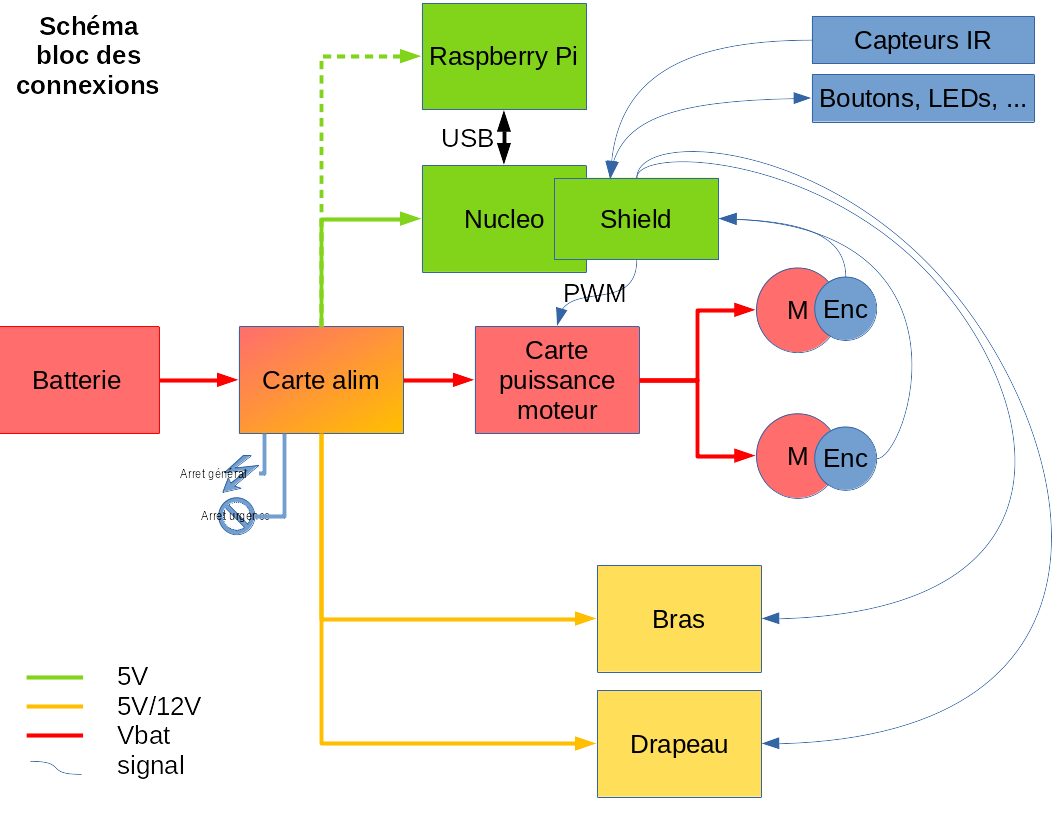
\includegraphics[scale=0.4]{schema_bloc_connexions.png}
  \caption{Schéma de principe de la carte d'alimentation}
\end{figure}
Les détails techniques sont disponibles dans le dossier
\href{https://github.com/eirbot/eirbot2020-1A/tree/master/alim}{alimentation}
sur github.
\begin{figure}[H]
  \center
  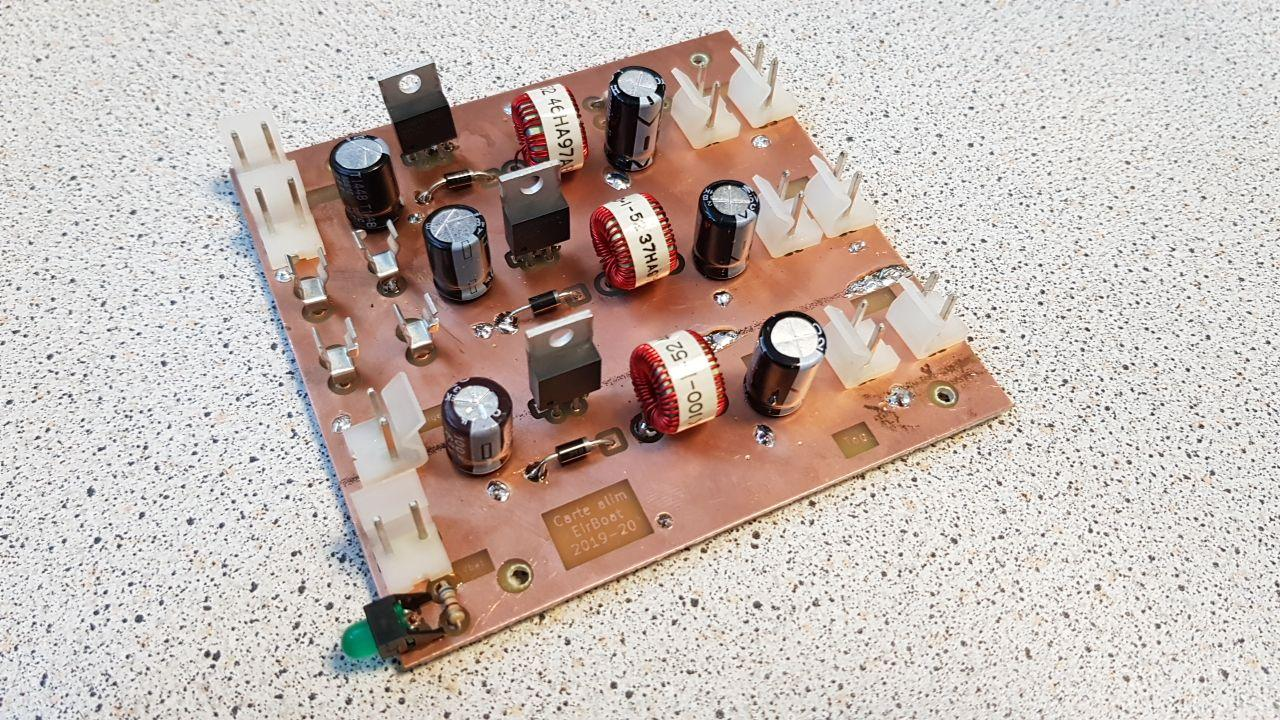
\includegraphics[scale=0.5]{alimentation.jpg}
  \caption{Résultat de la carte d'alimentation}
\end{figure}

\section{Puissance}
\paragraph{Objectif.} Les cartes de puissance permettent de récupérer
l'alimentation fournies par l'alimentation et de transmettre au moteur la bonne
puissance selon les commandes de l'asservissement. Elle permet aussi au moteur
de réaliser une marche arrière via un pont en H.
\paragraph{Mise en oeuvre.}

\paragraph{Résultat.}

\section{Actionneur}

\chapter{Informatique}
L'idée de cette partie est de donner un description de tous le soft que nous
avons mis en place. Cette partie est la plus volumineuse car c'est la plus
abstraite. Nous avons divisé ce chapitre en trois parties. Tout d'abbord une
partie Asservissement qui est basé sur la nucléo et qui permet d'envoyer de
réaliser les déplacements ``unitaire'' de robot. Dans un second temps nous avons
la partie Stratégie. Cette dernière est basée sur la raspberry et permet de
réaliser les calculs de trajectoire, les gestions des manoeuvres d'évitemment et
la comptabilisations des points. Finalement un protocole de communication permet
de garder un contact entre les deux cartes. \\
Il est à noter que nous avons réfléchis à un certain nombre de cas critiques
(perte de la communication rasp/nucléo etc) pour éviter de se retrouver bloqué
au milieu de la table.
\section{Asservissement}
\section{Stratégie}
\subsection*{Introduction}
Cette partie à pour objectif de définir de manière abstraite la communication
entre les différents blocs informatique pour permettre une compréhension
générale par tous (le violet représente le plus haut niveau, le vert représente
un point de communication avec la nucléo).
\begin{center}
  \begin{tikzpicture}
  \tikzstyle{lien}=[->,>=stealth,rounded corners=20pt,thick]
\tikzset{individu/.style={draw,thick,fill=#1!25},
individu/.default={white}, rounded corners=4pt}
\node[individu=violet] (A) at (0,0){\textsc{Main}};
\draw(1,0) node[right]{Envoie les ordres};
\draw(1,-0.5) node[right]{au fur et à mesure};
\node[individu=blue!50!black] (B) at (0,2){Navigation};
\draw(1,2) node[right]{$\leftarrow$ Calcul d'un};
\draw(1,1.5) node[right]{\; \; chemin précis};
\draw(-1,2) node[left]{Transformation en $\leftarrow$};
\draw(-1,1.5) node[left]{chemin global \;\;\;};

\node[individu=blue] (C) at (3,4){World};
\draw (4,4) node[right]{Renseigne position};
\draw (4,3.5) node[right]{obstacles};
\node[individu=green] (D) at (-3,4){Asservissement};
\draw (-4.5,4) node[left]{Permet d'envoyer};
\draw (-4.5,3.5) node[left]{requete déplacement};
\node[individu=blue!50!black] (E) at (-4,0){Evitemment};
\draw (-5,0) node[left]{Court circuite};
\draw (-5,-0.5) node[left]{le main};
\node[individu=green] (F) at (-3,-2){Détection};
\draw (-3,-2.5) node[below]{Renseigne GP2};
\node[individu=green] (G) at (3,-2){Actionneur};
\node[individu] (H) at (3,-4){Affichage};

\draw[lien] (A) -- (B);
\draw[lien] (A) -- (F);
\draw[lien] (A) -- (G);
\draw[lien] (F) -- (A);
\draw[lien] (B) -- (D);
\draw[lien] (C) -- (B);
\draw[lien] (E) -- (B);
\draw[lien] (F) -- (E);


  \end{tikzpicture}
\end{center}
\subsection{Modélisation de la table - Définition des obstacles}
\paragraph{Objectif.} Cette section de la stratégie est la première section,
elle a pour but de définir l'environnement dans lequel le robot va évoluer.
Cette définition de l'environnement sera cruciale pour la recherche de chemin.
L'objectif est donc de créer un système permettant de définir des obstacles et
des méthodes permettant de verifier si il y a des obstacles à un endroit.

\paragraph{Définition d'un obstacle.} La structure permettant de définir un
obstacle est relativement simple, elle contient la position du centre d'un
obstacle, sa largeur et sa longueur. Avec cette définition tous nos obstacles
sont rectangulaires. Par la suite, nous avons renseigné les positions de tous
les obstacles et leurs types (eco cup, petit taquet, grand taquet). Nous mettons
toutes ces informations dans un vecteur. Ce vecteur sera l'élément de base pour
détecter les collisions entre notre robot et les obstacles.

\paragraph{Prévision de collision.} L'idée est d'obtenir une méthode permettant
de savoir si notre robot peut aller à un point donné sans toucher d'obstacles.
Nous réalisons un test mathématique simple qui permet de nous donner en fonction
de coordonées $x,y$, d'une forme d'obstacle et d'une liste contenant tous les
obstacles si la case est valide ou non. Le fait de pouvoir tester les
différentes formes d'obstacles nous permet dans des cas critiques de désactiver
les tests sur les objets qui sont mobiles et ainsi nous sortir d'une situation
délicate. \\

\indent En somme nous disposons maintenant d'une modélisation simple de la table ce qui
nous permettra de pouvoir calculer les déplacements du robot tout en évitant les
obstacles. Nous ajoutons aussi une fonctionalité permettant de ne pas prendre en
compte toutes les obstacles ce qui nous permet de prioriser l'évitemment de
certains obstacles (nous préférons rentrer en collision avec une eco\_cup
qu'avec un robot).

\subsection{Recherche de Chemin - Algorithme A$\ast$}
\paragraph{Objectif.} L'idée est d'implémenter un algorithme permettant de
calculer un chemin pour notre robot. L'idée est qu'il puisse, d'un point donné
aller à un autre point tout en évitant les obstacles. Ces obstacles seront soit
défini directement (comme les gobelets) ou défini en fonction de la détection
des robots adverses. Nous réutilisons la classe \textit{world} pour
l'implémentation des obstacles.
\paragraph{Description de l'algorithme de pathfinding A*.}
A*\footnote{\url{https://fr.wikipedia.org/wiki/Algorithme_A*}} commence à un
nœud choisi. Il applique à ce dernier un cout initial, il estime ensuite la
distance entre ce noeud et le but à atteindre. Le coût additionné à l'évaluation
représentent le \textit{cout euclidien} assignné au chemin menant à ce noeud.
Le noeud est alors ajouté à une file d'attente prioritaire, appelée \textit{open
list}.

Premièrement l'algorithme récupère le premier noeud de l'\textit{open list}. Si
elle est vide, il n'y a aucun chemin du noeud initial à celui d'arrivé,
l'algorithme est en erreur. Si le noeud est celui d'arrivé, l'algorithme va
reconstruire\footnote{Cette reconstruction se fait grâce aux informations de la
  \textit{closed list}} le chemin complet et renvoyer le résultat.

Ensuite, si le noeud n'est pas le noeud d'arrivée alors de nouveaux noeuds sont
crées pour tous les noeuds contigus admissibles\footnote{Dans notre cas si il
  est libre ou non}. L'A$\ast$ calcule ensuite son coût et le stocke avec le
noeud. Ce coût est calculé à partir de la somme du coût de son ancêtre et du
coût de l'opération pour atteindre ce nouveau noeud.

En parallèle l'algorithme conserve la liste des noeuds qui ont été vérifiés,
c'est la \textit{closed list}. Si un noeud nouvellement produit est déjà dans
cette liste avec un coût égal ou inférieur, on ne fait rien.

Après, l'évaluation de la distance du nouveau noeud au noeud d'arrivée est ajoutée
au coût pour former l'heuristique du noeud. Ce noeud est alors ajouté à la liste
d'attente prioritaire, à moins qu'un noeud identique dans cette liste ne possède
déjà une heuristique inférieure ou égale.

Une fois ces étapes effectuées pour chaque nouveau noeud contigu, le noeud
original pris de la file d'attente prioritaire est ajouté à la liste des noeuds
vérifiés. Le prochain noeud est alors retiré de la file d'attente prioritaire et
le processus recommence.

\paragraph{Mise en oeuvre.} Les détails techniques sont disponibles dans le
dossier code, fichier
\href{https://github.com/eirbot/eirbot2020-1A/blob/master/code/src/navigation.cpp}{navigation}.
\\ Reprennons l'idée générale de cette partie : implémentation d'une recheche de
chemin. L'algorithme qui au coeur de cette recherche de chemin à déjà été
présenté. Nous allons donc décrire la classe \textit{Navigation}, le but de
cette classe est de récupérer une destination souhaitée, de trouver le chemin
(tout en évitant les obstacles) via l'A* et enfin d'effectuer les déplacements
en appelant la classe d'Asservissement via le protocole de
communication.\\ Cette classe aura donc des noeuds comme attribut, (un noeud
contient la position $x,y$, les différents cout $fcost, gcost, hcost$ et les
parents du noeud $parentX,parentY$). Elle possède 3 méthodes principales, tout
d'abord Astar qui permet d'executer l'Astar, cette méthode appelle MakePath qui
a pour but de construire un vecteur contenant le chemin final. Cepedant à ce
stade nous avons une description du chemin très précise (centimètre par
centimètre), nous devons fournir quelque chose de moins précis à
l'asservissement (au risque d'avoir un papybot). Pour cela nous avons la méthode
NavigateToAsserv qui permet de transformer ce chemin en suite de segment ce qui
nous permet de nous déplacer.\\ A ce stade nous avons un moyen de trouver notre
chemin et faire deplacer un robot de manière assez brutale, il faudrait
développer un algorithme de lissage de la trajectoire (pour avoir des
changements de direction moins brutaux).

\subsection{Détection des adversaires}
\paragraph{Objectif.} L'idée de cette partie est de montrer comment nous avons
utilisé les différents détecteurs (GP2) pour mettre au point un système de
détection et surtout de réaction pour la détection. Dans un premier temps nous
avons pensé à court circuiter la nucléo et la rasp lorsque nous avons une
interuption de détection. Nous avons ensuite trouvé un moyen de l'intégrer dans
la boucle principale.
\paragraph{Mise en oeuvre.} Le code de haut niveau est relativement simple, il
consiste à utiliser la définition des obstacles. Lorsque nous détectons un robot
adverse, la stratégie prend un branchement, récupère l'information sur la
distance par rapport au robot et place un obstacle de la taille d'un robot puis
relance la navigation ce qui permet d'éviter l'obstacle. A la fin du branchement
l'obstacle est détruit. Il s'agit maintenant de transmettre l'information entre
les GP2, la nucléo et la raspberry. En parallèle de la détection ``normale''
nous allons réutiliser le point que nous avons soulevé lors de la définition des
obstacles c'est à dire le fait que nous pouvons supprimer des obstacles. En
effet supposons que nous détectons un robot, nous plaçons un nouvel obstacle
puis nous relançons la navigation. Cependant le nouvel obstacle pourrait
conduire à un échec de la navigation, notre robot peut être dans le cas où il
est bloqué. Nous créons alors une autre étape dans notre branchement. Lorsque
nous relançons la navigation si cette dernière ne trouve pas de chemin car nous
sommes bloqué alors nous enlevons tous les obstacles du type ``eco cup''. Cela
nous permet alors de nous sortir de notre situation de bloquage (tout en
poussant des eco cup). A ce stade nous avons un système permettant de détecter
et de réagir lorsque nous avons un robot adverse face à nous.

Nous allons maintenant décrire comment
s'organise la communication.
\subsection{Gestion des actionneurs}
\subsection{Boucle de jeu principale}
\subsection{Mise en place de tests}
\paragraph{Objectif.}

\section{Protocole de communication Stratégie $\rightarrow$ Asservissement}
\subsection{Asservissement}
Commençons par le cas d'utilisation classique, nous estimons que la nucléo ne
rencontre aucun problème particulier. Dans ce cas normal la rasp peut envoyer
trois types de requêtes, une de position, une d'angle et une d'initialisation.
Le protocole de communication transforme ces requêtes en instructions pour la
nucléo. La nucléo execute les actions et renvoie une confirmation d'execution de
la requete ce qui informe la rasp que l'action a correctement été réalisée.
\\ Dans un second temps nous présentons le mécanisme qui se met en place si la
rasp transmet un ordre mais qu'aucune réponse n'est receptionnée sur une action.
\\
\begin{multicols}{2}
\begin{center}
  \begin{tikzpicture}
  \tikzstyle{lien}=[->,>=stealth,rounded corners=20pt,thick]
\tikzset{individu/.style={draw,thick,fill=#1!25},
individu/.default={white}, rounded corners=4pt}
\node[individu] (A) at (0,0){\textsc{Rasp}};
\node[individu] (B) at (0,-3){\textsc{Communication}};
\node[individu] (C) at (0,-6){\textsc{Nucléo}};

\draw[lien] (A) -- (-1,-2.75);
\draw (-0.5,-1.375) node[left]{$x,y$};
\draw[lien] (-1,-2.75) -- (A);

\draw[lien] (A) -- (0,-2.75);
\draw (0,-1.375) node[left]{$\theta$};
\draw[lien] (0,-2.75) -- (A);

\draw[lien] (A) -- (1,-2.75);
\draw (0.5,-1.375) node[right]{position};
\draw[lien] (1,-2.75) -- (A);

\draw[lien] (-1,-3.25) -- (C);
\draw (-0.5,-4.625) node[left]{go\_to};
\draw[lien] (-1,-3.25) -- (C);

\draw[lien] (0,-3.25) -- (C);
\draw (0,-4) node[left]{angle};
\draw[lien] (0,-3.25) -- (C);

\draw[lien] (1,-3.25) -- (C);
\draw (0.5,-4.625) node[right]{position};
\draw[lien] (1,-3.25) -- (C);

  \end{tikzpicture}
\end{center}
\columnbreak

\begin{center}
  \begin{tikzpicture}
    \tikzstyle{lien}=[->,>=stealth,rounded corners=20pt,thick]
    \tikzstyle{lien2}=[->,>=stealth, rounded corners=20pt, thick,red]
\tikzset{individu/.style={draw,thick,fill=#1!25},
individu/.default={white}, rounded corners=4pt}
\node[individu] (A) at (0,0){\textsc{Rasp}};
\node[individu] (B) at (0,-3){\textsc{Communication}};
\node[individu] (C) at (0,-6){\textsc{Nucléo}};

\draw[lien] (A) -- (-1,-2.75);
\draw (-0.5,-1.375) node[left]{$x,y$};

\draw[lien2] (-1,-2.75) -- (0,-1.5) -- (A);
\draw (-0.5,-1) node[left,red]{timeout};

\draw[lien] (-1,-3.25) -- (C);
\draw (-0.5,-4.625) node[left]{go\_to};

\draw[lien] (A) -- (0.5,-2.75);
\draw (0.5,-1) node[right]{position};
\draw[lien] (A) -- (0.5,-2.75);

\draw[lien] (1,-3.25) -- (C);
\draw (0.5,-4.625) node[right]{position};
\draw[lien] (C) -- (1,-3.25);

\draw[lien] (A) -- (1,0) -- (0,1) -- (A);
\draw (0.5,0.5) node[right]{new\_calcul};

  \end{tikzpicture}
\end{center}
\end{multicols}
Il faut encore gérer le cas ou la nucléo ne répond plus du tout, nous réalisons
alors un branchement, si nous obtenons une succession de timeout alors nous
arretons la rasp et nous lançons un programme d'urgence pour que la nucléo
fasse un programme minimal (c'est à dire rentrer au port). Nous devons encore définir comment activer ce
programme minimal.

\subsection{Détection}
Le protole de communication pour la détection va fonctionner de manière très
similaire à l'asservissement. La principale différence réside dans le fait que
la nucléo peut envoyer une interuption à la rasp pour lui indiquer que l'on
détecte un robot adverse. \\
Dans le cas d'une détection, automatiquement la nucléo va stopper les moteurs et
envoyer à la rasp l'information via le protocole de communication. La rasp va
alors recevoir les informations de tous les GP2 actifs sur les différentes
distances seuils. Une fois cela effectué, la rasp va déterminer la position et
l'angle du robot, elle va alors pouvoir créer un nouvel obstacle et recalculer
une trajectoire tout en évitant le robot. Si l'on évite correctement le robot
adversaire nous continuons notre trajectoire. Dans le cas contraire, les GP2
redetecte quelque chose, la nucléo renvoie une interuption etc. Si l'on arrive
dans un cas de figure où nous avons des interuptions sans arret alors nous
réalisons une manoeuvre d'évitement de grande ampleur. Qui consiste à reculer et
faire un détour pour être sur de l'éviter. \\
Il reste un dernier cas à traiter si lorsque nous détectons un robot et que la
navigation de la rasp ne trouve pas de chemin. Dans ce cas nous devons tout de
même nous sortir de la situation. Ainsi la navigation va supprimer les obstacles
du type eco\_cup et s'échapper tout en renversant les écocups. \\
Ainsi nous avons théoriquement un système qui nous permet de détecter et
d'éviter un robot adverse.

\end{spacing}
\end{document}
